
% What is the problem?

The model-checking needed by correct-by-construction controllers could limit the scalability of 
autonomy.  Model-checking generates controllers, validates correctness, and ensures performance based on 
an exploration of the state-space of a finite model system.   As autonomy scales, so does the 
state space, making it impossible to evaluate models that describe the entire system. 

To avoid the explosion of state, systems must be decomposed into networks and hierarchies of 
interacting components that represent systems at multiple scales.  Decomposition of
a system into parts can be done by data, task, actor, or localization.
% How do you propose to solve it?

This approach to scalability inherits from service-oriented architectures used to build 
Internet and Cloud software 
in which complex systems are assembled from multiple simple services with well-defined interfaces.
Software systems built in this manner are agile; they may be updated, modified or patched incrementally.  
Modifications are deployed directly into the running system after validation against the interface
specification.  Often they are deployed to small fractions of the total system for testing on the 
operational system.  Modifications are rolled back if they disrupt function.
This is in contrast to monolithic software engineering processes in which 
entire systems are built, verified, validated, and deployed.  The time to deploy any new function
in monolithic software grows with system complexity and systems quickly become unmanageable. 

\begin{figure}
\begin{center}
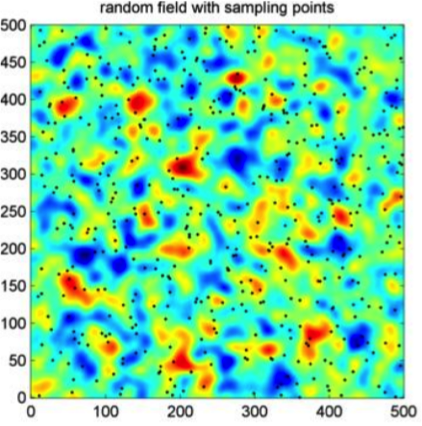
\includegraphics[height=2in]{kriginga.png} 
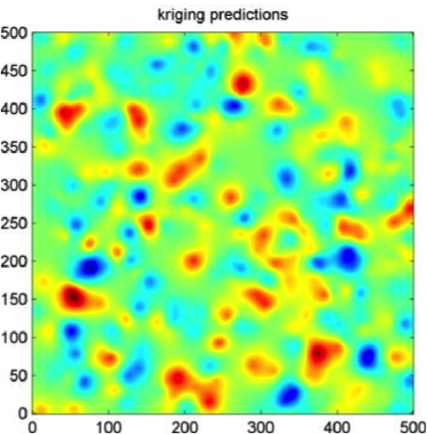
\includegraphics[height=2in]{krigingb.png} 
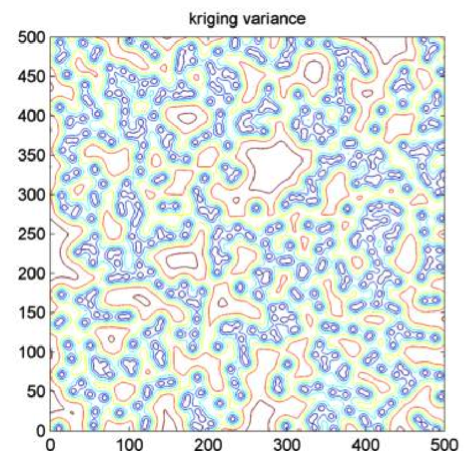
\includegraphics[height=2in]{krigingc.png} 
\end{center}
\caption{A heatmap visualization of a random field to be sensed and the sampling points, i.e. the present locations of the UAVs (left).
  The approximation of the field based on kriging (Gaussian process estimation) of the current sensor locations (center).  
  The error in the sensed field (right).
  Images from {\small \url{http://www.mathworks.com/matlabcentral/fx_files/29025/1/kriging.jpg}}.} 
\label{fig:krig}
\end{figure}

We provide an abstract example that demonstrates how a system-wide goal can be 
achieved hierarchically by a network of independently autonomous actors coordinating 
locally with other system elements.  The example is one of autonomously navigating UAVs of sensing an infra-red 
spatial field to specified accuracy, i.e. to a maximum known error across the sensing space.
The example leverages a Gaussian process estimation technique, known as kriging, to localize 
information and allow the sensors to act independently or in small groups.  Kriging has the 
property that it estimates a field based on a finite number of sensors and, more importantly, 
provides known error on the field estimate.  Figure \ref{fig:krig} shows this process, demonstrating
the original field and sensor locations (left), the estimated field (center), and the  known error in the
estimate (right).  Because the estimate for the field has local support, sensors communicating locally
with a small set of other sensors can determine an overestimate of the local error.  They use
this information to autonomously navigate to regions of high error, which will drive down global
error.  Figure \ref{fig:krig2} shows one possible navigation strategy used by a small group collaborating 
based on local information.  They use a greedy approach in which they navigate to closest areas 
of high error.   Navigation will continue, monotonically decreasing error in the field, until the 
goals have been met.

\begin{figure}
\begin{center}
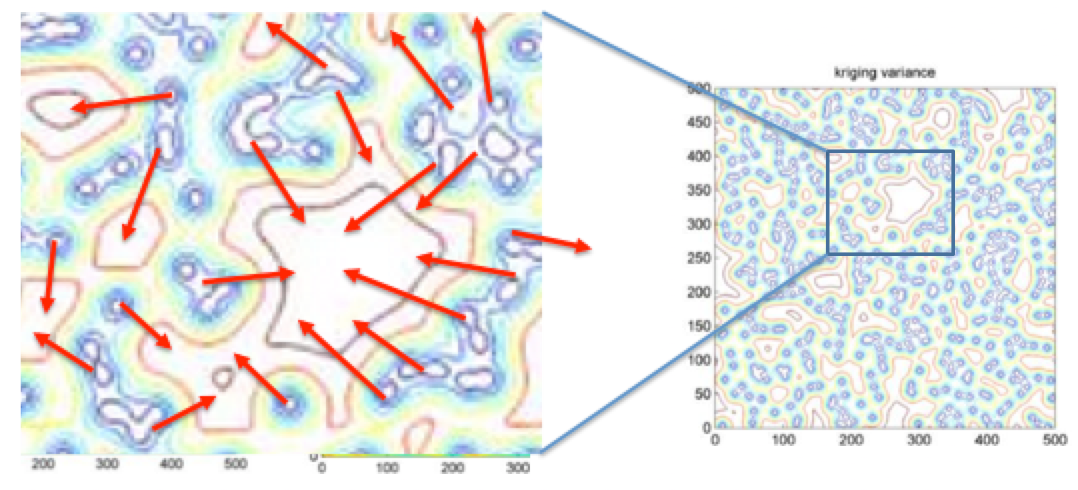
\includegraphics[height=2.7in]{krigingd.png} 
\end{center}
\caption{UAVs navigating to regions of high error based on local information when collaboratively sensing a field.
  Original images from {\small \url{http://www.mathworks.com/matlabcentral/fx_files/29025/1/kriging.jpg}}.  The
  zoom effect and the motion of sensors indicated by arrows have been added.} 
\label{fig:krig2}
\end{figure}

This example demonstrates desirable properties of autonomous systems that will achieve scale:  
it is {\em goal-based} and {\em declarative}.  With goal-based autonomy, one expresses the  
objective of the system in a simple statement, in this case, sense the field with known error.  
Goal-based autonomy allows us to assemble multiple autonomous systems in hierarchies and networks.
The simplicity of the goal means that this autonomous subsystem has a well known interface for 
other systems that want to consume its output.  Describing the outcome of a complex system in a 
simple goal will allow multiple such systems to interact and will be necessary to scale 
autonomy to the battlespace.  Declarative indicates that the subsystem is tasked by a statement 
of {\em what to do} rather than {\em how to do it}.  This allows the subsystem to self-optimize,
choosing from among many possible execution strategies based on local knowledge.  Declarative 
strategies compartmentalize complexity, allowing each system to use the high-resolution data
needed to accomplish its goal, but hide that complexity from the overall system.
